\cleardoublepage

\chapter{Diseño de la solución}

La solución propuesta \ref{sec:motivacion} se ha desarrollado siguiendo las siguientes fases: una primera etapa de preparación de
entorno seguro, una segunda etapa de identificación, y una final de autenticación. Para cada una de las fases se adjunta una 
diagrama de secuencias \footnote{Los valores entre $<$ y $>$ indican un valor en concreto, no el valor definido entre ambos 
símbolos} \footnote{Los tópicos tienen la estructura emisor/receptor/item}

\section{Fase TLS}
\label{sec:tls_phase}

En esta fase, el broker MQTT debe crear un certificado firmado por una CA para verificar su identidad. 
Para comunicarse por TLS con el broker MQTT, se ha llevado a cabo los siguientes pasos:

\begin{enumerate}
    \item Crear la clave privada de la \acrshortpl{ca}
    \item Crer el certificado CA usando la clave privada del paso 1 para firmarla
    \item Crear la clave privada del broker MQTT
    \item Crear la solicitud de firma de certificados (\acrshort{csr}) para el broker MQTT usando la clave privada del paso 3
    \item Usar la clave y certificado CA para firmar el certificado del broker MQTT
    \item Distribuir la clave y certificado en la CA
    \item Distribuir el certificado CA a los cliente que se quieran comunicar a través del broker MQTT 
\end{enumerate}

\begin{figure}[H]
    \centering
    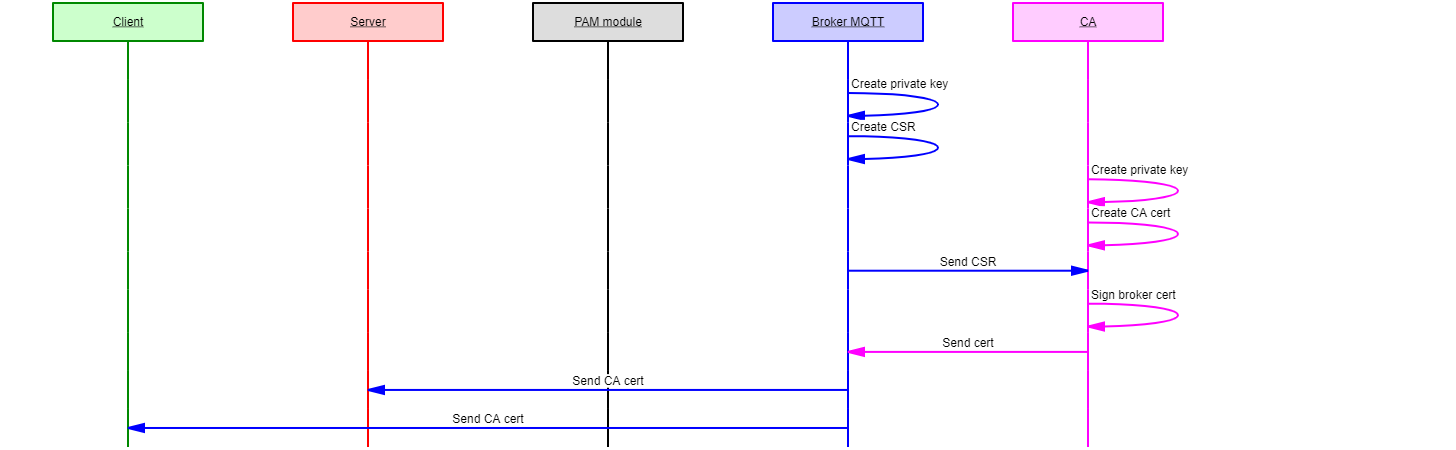
\includegraphics[scale=0.25]{tls_phase.png}
    \caption{Fase TLS}
\end{figure}

Como último paso, el archivo de configuración del cliente \textit{mosquitto} en el broker MQTT tiene que indicar la clave y 
certificados necesarios tal y como figura en \ref{code:pam_conf}.

Si un cliente quiere usar el broker MQTT para publicar un mensaje o subscribrse a un tópico, necesita ``mostrar'' el certificado
CA al broker MQTT. No es la única forma de identificación vía TLS. También existe la opción de que cada cliente
cree su propio certificado firmados por la CA.

\section{Fase de identificación}
\label{sec:id_phase}

En esta fase, el cliente se tiene que registrar en el servidor para poder usar su servicio. Para ello, el cliente crea un 
identificador único \acrfull{uuid} y un par de claves pública y privada. Estos se guardan en un directorio en concreto. Se ha
escogido \textit{.anubis} en la carpeta \textit{home} del usuario. Las claves se guardan con el UUID como nombre del archivo y
finalmente se envía la clave pública al servidor. Se puede usar el protocolo \acrfull{scp}. Dado que no se quiere usar un método
de autenticación distinto al propuesto por este trabajo, se podría crear una clave pública temporal del servidor y subirla a 
algún servidor de claves públicas. El cliente por tanto podría usarla para mandar su clave pública a su directorio \textit{.anubis} 
de forma segura y una vez envíada,  

Una vez que el servidor tiene la clave pública del cliente, este primero revocaría la clave pública del servidor de claves y 
posteriormente lo registra en el archivo de configuración de usuario \ref{code:user_conf}. Este indica el UUID concreto para un 
usuario en el sistema. Se usa en caso de que el usuario tenga varias claves públicas y por tanto el servidor sepa que clave usar 
para la autenticación.

\begin{figure}[H]
    \centering
    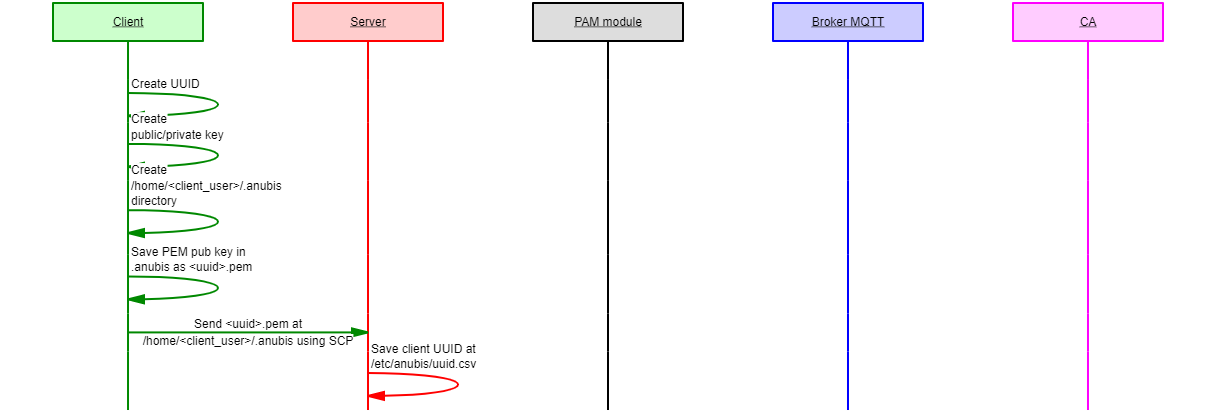
\includegraphics[scale=0.25]{id_phase.png}
    \caption{Fase de identificación}
\end{figure}

\section{Fase de autenticación}

En esta fase reside el proces de autenticación del cliente contra el servidor una vez que se ha establecido un canal seguro y 
registrado el cliente en el servidor.

El cliente se subscribe al tópico \textit{pam/$<$uuid$>$/challenge} por el cual recibirá el desafío y envía una petición de para 
abrir una sesión por SSH. 

Al llegar la petición SSH al servidor, este comprueba el UUID del usuario que se quiere autneticar en el 
archivo de configuración de ususarios \ref{code:user_conf}. Una vez el servidor conoce el UUID, de plantean dos posibilidades:

\begin{enumerate}
    \item Que el usuario no necesite autenticarse de la forma propuesta
    \item Que el usuario tenga que autenticarse
\end{enumerate}

Cada condición se da según la política definida en el archivo de configuración de anubis \ref{code:anubis_conf}. Existen dos 
tipos de políticas:

\begin{enumerate}
    \item \textit{relax}: no es necesario aplicar la autenticación
    \item \textit{strict}: se aplica la autenticación
\end{enumerate}

La política \textit{relax} es útil en casos en los que por ejemplo el usuario provenga de una red de confianza como puede ser una
Universidad. En ese caso, el módulo PAM propuesto devolvería un \textit{PAM\_IGNORE} pasando el siguiente módulo. En caso de la 
política \textit{strict}, es necesario pasar el proceso de autenticación propuesto y que devuelva un \textit{PAM\_SUCCESS}.

Para una política \textit{strict}, el servidor se subscribe a dos tópicos por los cuales el cliente publicará el par de valores 
[$r, s$] del algoritmo ECDSA definido en \ref{subsec:ecdsa} en formato hexadecimal:

\begin{itemize}
    \item \textit{$<$uuid$>$/pam/r}
    \item \textit{$<$uuid$>$/pam/s}
\end{itemize}

Crea el desafío y lo publica al tópico \textit{pam/$<$uuid$>$/challenge}. Al llegar el mensaje al broker MQTT, este lo reenvía a todos
los nodos que estén suscritos a dicho tópico. Dado que solo hay un UUID por cliente, el mensaje solo le llega al cliente 
determinado por el UUID. 

El cliente crea el hash del desafío. Concretamente, para este proyecto se ha usado el algoritmo SHA-512 dada su robustez con 
respecto a otros de menor tamaño como puede ser SHA-256. Una vez que tiene el hash, lo firma usando su clave privada creada en
\ref{sec:id_phase} y envía ambos valores $[r,s]$ por los tópicos \textit{$<$uuid$>$/pam/r} y \textit{$<$uuid$>$/pam/s} respectivamente
siendo estos retransmitidos por el broker MQTT al servidor ya que es el único que conoce el UUID del cliente.

Finalmente, el servidor general el hash del desafío y junto a la clave pública del cliente verifica que el hash es correcto y 
está firmado por el cliente verídico. Si es verídico, el servidor devuelve \textit{PAM\_SUCCESS}. En caso contrario, 
\textit{PAM\_AUTH\_ERR}.


\begin{figure}[H]
    \centering
    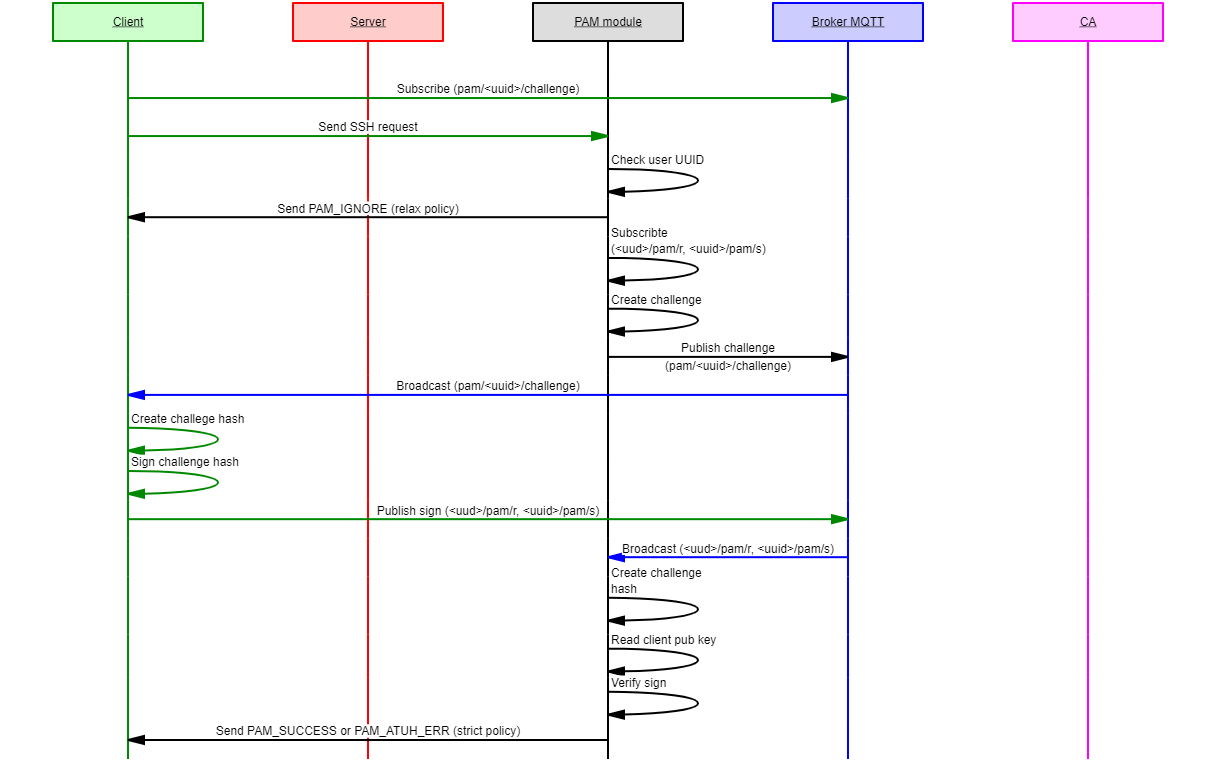
\includegraphics[scale=0.25]{auth_phase.png}
    \caption{Fase de autenticación}
\end{figure}


En la siguiente imagen se mustra la topología global del sistema propuesto:

\begin{figure}[H]
    \centering
    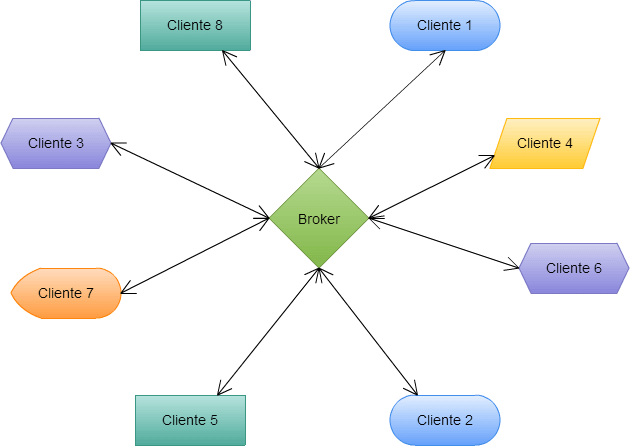
\includegraphics[scale=0.15]{topologia.png}
    \caption{Topología del diseño}
\end{figure}

\section{Código fuente}

El código fuente no se adjunta por simplicidad y limpieza en la memoria pero se encuentra subido a la plataforma de GitHub 
\cite{garcia_sergiogp98mqtt-pam_2021}. 